%\subsection{System Validation}

To validate the stimulation and data acquisition system design, a standard electrophysiology experiment, described in~\cite{Olivo,KuehJellies,EllingerMSEE}, was performed on earthworm giant axon action potentials, henceforth referred to as the Earthworm Experiment.  This serves the purpose of showing that the Data Acquisition and Stimulation System is capable of being used in an electrophysiology experiment, and the procedure has been performed with previous designs, allowing the new design to be compared with previous results~\cite{StahlMSEE}.

%The earthworm's nerve fibers do not have a myelin sheath like many larger animals.  A myelin sheath insulates the ionic solution outside of the nerve fiber and results in faster propagation of an electric potential along the length of the fiber.  Without the myelin sheath the earthworm can not quickly propagate instructions to its muscles, which inhibit its response to dangers in its environment.  To overcome this limitation, there are giant axons along its nerve cord that are bundles of nerve fibers that each transmit the same information.  This arrangement results in faster propagation of the electric potential allowing the earthworm to quickly respond to danger.

In the earthworm's nerve cord, there is a median giant axon and two smaller lateral giant axons on either side of the median axon.  The lateral giants are connected to each other at multiple locations along the length of the earthworm which has the effect of lateral axons acting as a single giant axon~\cite{Olivo}.  A physical or electrical stimulation near the anterior or posterior ends of the earthworm will elicit a response from the earthworm in the form of an action potential that propagates along one or both of the giant axons.  The propagation speed is related to the cross sectional area of the axon~\cite{KuehJellies}.  Varying the intensity of the electrical stimulation at the anterior end of the earthworm will show no response at low intensity, an action potential along the median axon soon after the stimulation at medium intensity, and at a higher intensity, action potentials along both the median and lateral giant axons will be visible with the median response occurring sooner than the lateral response due to the differing propagation speeds.  Figure~\ref{fig:EWCrossSec} shows a cross section of an earthworm based on a figure in~\cite{Kladt2010} with a more detailed representation of the nerve cord based on~\cite{KuehJellies}.

\begin{figure}[H]
	\begin{singlespace}
	\centering 
		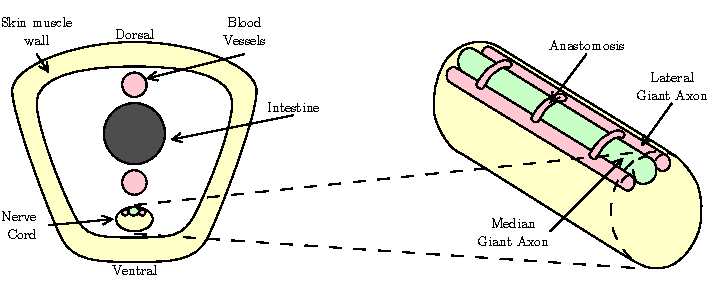
\includegraphics{./figures/EWCrossSec} 
	\caption{Cross section of an earthworm adapted from~\cite{KuehJellies,Kladt2010}\label{fig:EWCrossSec}}
	\end{singlespace}
\end{figure}


Electrical stimulation is accomplished by placing two pins near the anterior end of the earthworm.  Measurement of the action potentials along the axon is accomplished by dissecting the earthworm and placing two chlorided silver extracellular electrodes on the earthworm nerve cord.  The extracellular electrodes measure the difference in electric potential at two points on the nerve cord.  When an action potential propagates along the nerve cord, the electrodes measure a difference in voltage in time that will appear as a biphasic spike.  The exact shape of the spike will depend on the placement and size of the electrodes and the condition of the nerve cord itself~\cite{Olivo,KuehJellies,McGillCAP}.

The Data Acquisition and Stimulation System was used to perform an experiment studying earthworm giant axon action potentials with a previously developed and validated amplifier~\cite{StahlMSEE} and oscilloscope connected in parallel with the electrophysiology interface board, allowing the data to be compared.

\subsection{Earthworm Setup}

The dissection of the earthworm and setup of the stimulation and recording hardware is based on~\cite{Olivo,KuehJellies,StahlMSEE}.  Two pins are placed near the anterior end of the earthworm.  Connected to these pins is the output of the stimulation circuitry. Near the middle of the earthworm, the skin is cut and folded to expose the interior of the worm.  The intestine is moved out of the way, and the nerve cord is pulled away from the fluids with two chlorided silver electrodes that are connected to the amplification and recording circuitry. Between the stimulation pins and recording electrodes, a chlorided silver wire is placed under the body of the earthworm and connected to circuit ground, which may be connected to earth ground depending on the circuit setup.  Figure~\ref{fig:EWSetup} is a diagram of the DASS connected to the earthworm

\begin{figure}[H]
	\begin{singlespace}
	\centering 
		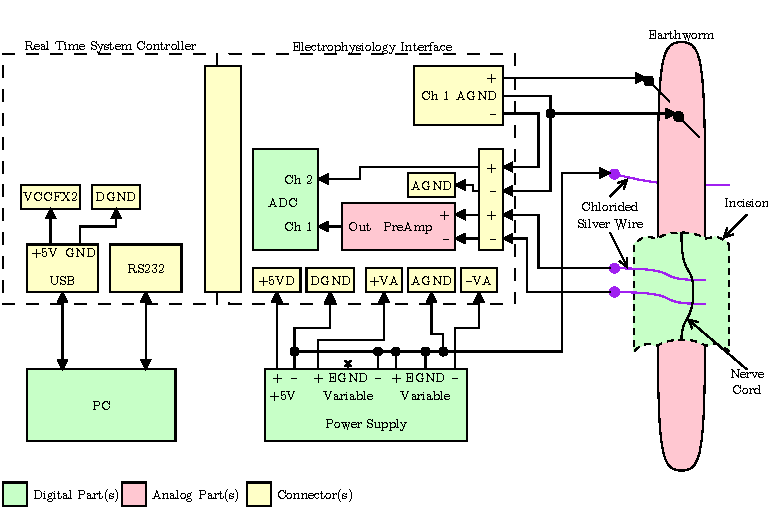
\includegraphics{./figures/EWSetup} 
	\caption{Diagram showing connections between the Data Acquisition and Stimulation System and an earthworm, connections to earthworm follow~\cite{Olivo,KuehJellies}\label{fig:EWSetup}}
	\end{singlespace}
\end{figure}

To compare the Data Acquisition and Stimulation System with a previously validated setup, the  Preamp from~\cite{StahlMSEE,BatzerCorsiCrampton}, with its output connected to an oscilloscope, has its input connected in parallel with the recording electrodes as shown in Figure~\ref{fig:EWSetupPA}.

\begin{figure}[H]
	\begin{singlespace}
	\centering 
		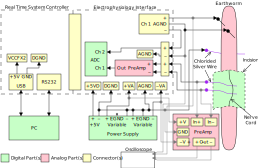
\includegraphics{./figures/EWSetupPA} 
	\caption{Diagram of the Data Acquisition and Stimulation System connected in parallel with a previously validated recording system, connections to the earthworm follow~\cite{Olivo,KuehJellies} and connections to the standalone Preamp and oscilloscope follow~\cite{StahlMSEE}\label{fig:EWSetupPA}}
	\end{singlespace}
\end{figure}

\subsection{Chloriding Silver Wire}

The silver wire used for the extracellular electrodes must be coated in a layer of silver chloride.  To create the coating, electroplating may be used as described in~\cite{KuehJellies,WarnerChloriding}. A simpler method is to place the portion of the wire that will be in contact with living tissue in full-strength Clorox\textsuperscript{\textregistered} bleach and leave the wire in the bleach until the wire acquires a purplish-gray tint, which should take between ten and thirty minutes~\cite{WarnerChloriding}.
 
\subsection{Earthworm Experiment Procedure}

The Earthworm Experiment procedure is adapted from~\cite{Olivo,KuehJellies}.

\subsubsection{Earthworm Dissection}

\begin{itemize}

\item Place the earthworm in a 10\% ethanol solution to anesthetize it

\item Leave the worm in the ethanol solution for the minimum amount of time needed to make the worm easy to work with while dissecting it; 5-10 minutes may be all that is necessary

\item Rinse the earthworm in tap water and pin it, dorsal (dark) side up, on the dissecting dish

\item Create a capital-letter-I shaped incision, using surgical scissors, one to two inches long, along the length of the worm, about halfway between the anterior and posterior ends of the earthworm

\item Pin the skin to the dissecting dish to expose the worm internal anatomy

\item Flush the cavity periodically, as needed, with worm Ringer's solution (in mM units: 102.7 NaCl, 1.6 KCl, 1.8 CaCl$_2$, and 4 NaHCO$_3$~\cite{KuehJellies}) to make the anatomy easier to view

\item Move the intestine aside, using forceps and scissors, exposing the nerve cord

\item Free a few centimeters of the nerve cord from its lateral and ventral connections, using the forceps and scissors, to allow the cord to be lifted above and away from the saline and other anatomy

\item Position the chlorided silver wires under the nerve cord

\item Raise the fixture holding the silver wires until the wires and nerve cord are away from the saline and earthworm anatomy (a fraction of an inch is all that is necessary, blowing in the area can break up the surface tension if the saline solution is bridging the wires and cord with the rest of the earthworm)

\item Moisten the nerve cord with Ringer's solution, often, throughout the experiment while making sure that the nerve cord and electrodes remain isolated from the rest of the saline and anatomy (it may be necessary to remove excess Ringer's solution)

\end{itemize}

\subsubsection{Electrical Setup}

\begin{itemize}

\item Place two pins near each other in the anterior end of the earthworm

\item Connect the non-inverting output of the stimulation circuit to one pin and connect circuit ground or the inverting output to the second pin

\item Connect, optionally, if the inverting output is not connected to a pin in the earthworm, the inverting output of the stimulation circuit to an unused electrode input channel on the Electrophysiology Interface board; ensure that there is no Preamp board in the PCI-Express socket and bypass the socket wiith a $0\Omega$ resistor.  See Figures~\ref{fig:EWSetup} and~\ref{fig:EWSetupPA}  

\item Place a chlorided silver wire under the body of the earthworm, between the stimulation pins and the exposed portion of the earthworm's body and connect the wire to circuit (which may be earth) ground

\item Connect the chlorided silver recording electrodes to the Preamp inputs with the non-inverting input connected toward the anterior end of the earthworm and the inverting input connector toward the posterior end (reversing the electrodes will simply invert the signal) (connecting the electrodes may be performed before the silver wires are placed under the nerve cord, to avoid disturbing the electrodes in the process of making the connections)

\item Power on the Electrophysiology Interface, first, then power on the RTSC

\end{itemize}

\subsubsection{Software Setup}

\begin{itemize}

\item Update FPGA program as described in~\cite{BatzerMSEE}

\item Update Cypress EZ-USB firmware as described in~\cite{BatzerMSEE}

\item Create the script and corresponding waveform file as shown in~\cite{BatzerMSEE}

\item Launch Data Acquisition and Stimulation Control Center (DASCC)

\item Select the appropriate COM port from the dropdown list

\item Select the appropriate Endpoint from the dropdown list, set Packets Per Xfer to 64, and set Xfers to Queue to 64

\item Select the Scripting tab and load the Earthworm Script as described in~\cite{BatzerMSEE}

\item When prepared for single stimulus and capture click the ``Run Script'' button.  Changes to the output pulse amplitude can be accomplished by changing the 2nd line of the Waveform file as shown in~\cite{BatzerMSEE}

\item Graph data by selecting the Graphing tab and clicking the ``Load File'' button.  Once loaded, multiple channels can be displayed at the same time using ctrl + left mouse button to select/deselect channels.

\item Click ``Output CSV'' to export data to a comma-separated values (CSV) text file

\end{itemize}

\subsubsection{Stimulation and Recording}

\begin{itemize}

\item Stimulate the earthworm with a single, $0.2\unit{ms}$ wide pulse with low amplitude (less than $1.0\unit{V}$)

\item Repeat the stimulation while slowly increasing the pulse amplitude (in steps between $0.1\unit{V}$ and $0.5\unit{V}$) until a response is seen between $2\unit{ms}$ and $8\unit{ms}$ after the stimulation artifact, this is the median giant response

\item Save the recorded waveform

\item Slowing increase the pulse amplitude, further, until a second response is seen between $6\unit{ms}$ and $15\unit{ms}$ after the stimulation artifact, this is the lateral giant response

\item Save the recorded waveform

\end{itemize}

\subsection{Results}\label{sec:results}

The Earthworm Experiment was performed with the Data Acquisition and Stimulation System connected in parallel with a preamp and oscilloscope that was validated in~\cite{StahlMSEE}.  A diagram of the experimental setup is shown in Figure~\ref{fig:EWSetupPA}.  A picture of the experimental setup is shown in Figure~\ref{fig:EWSetupPic}.

\begin{figure}[H]
	\begin{singlespace}
	\centering 
		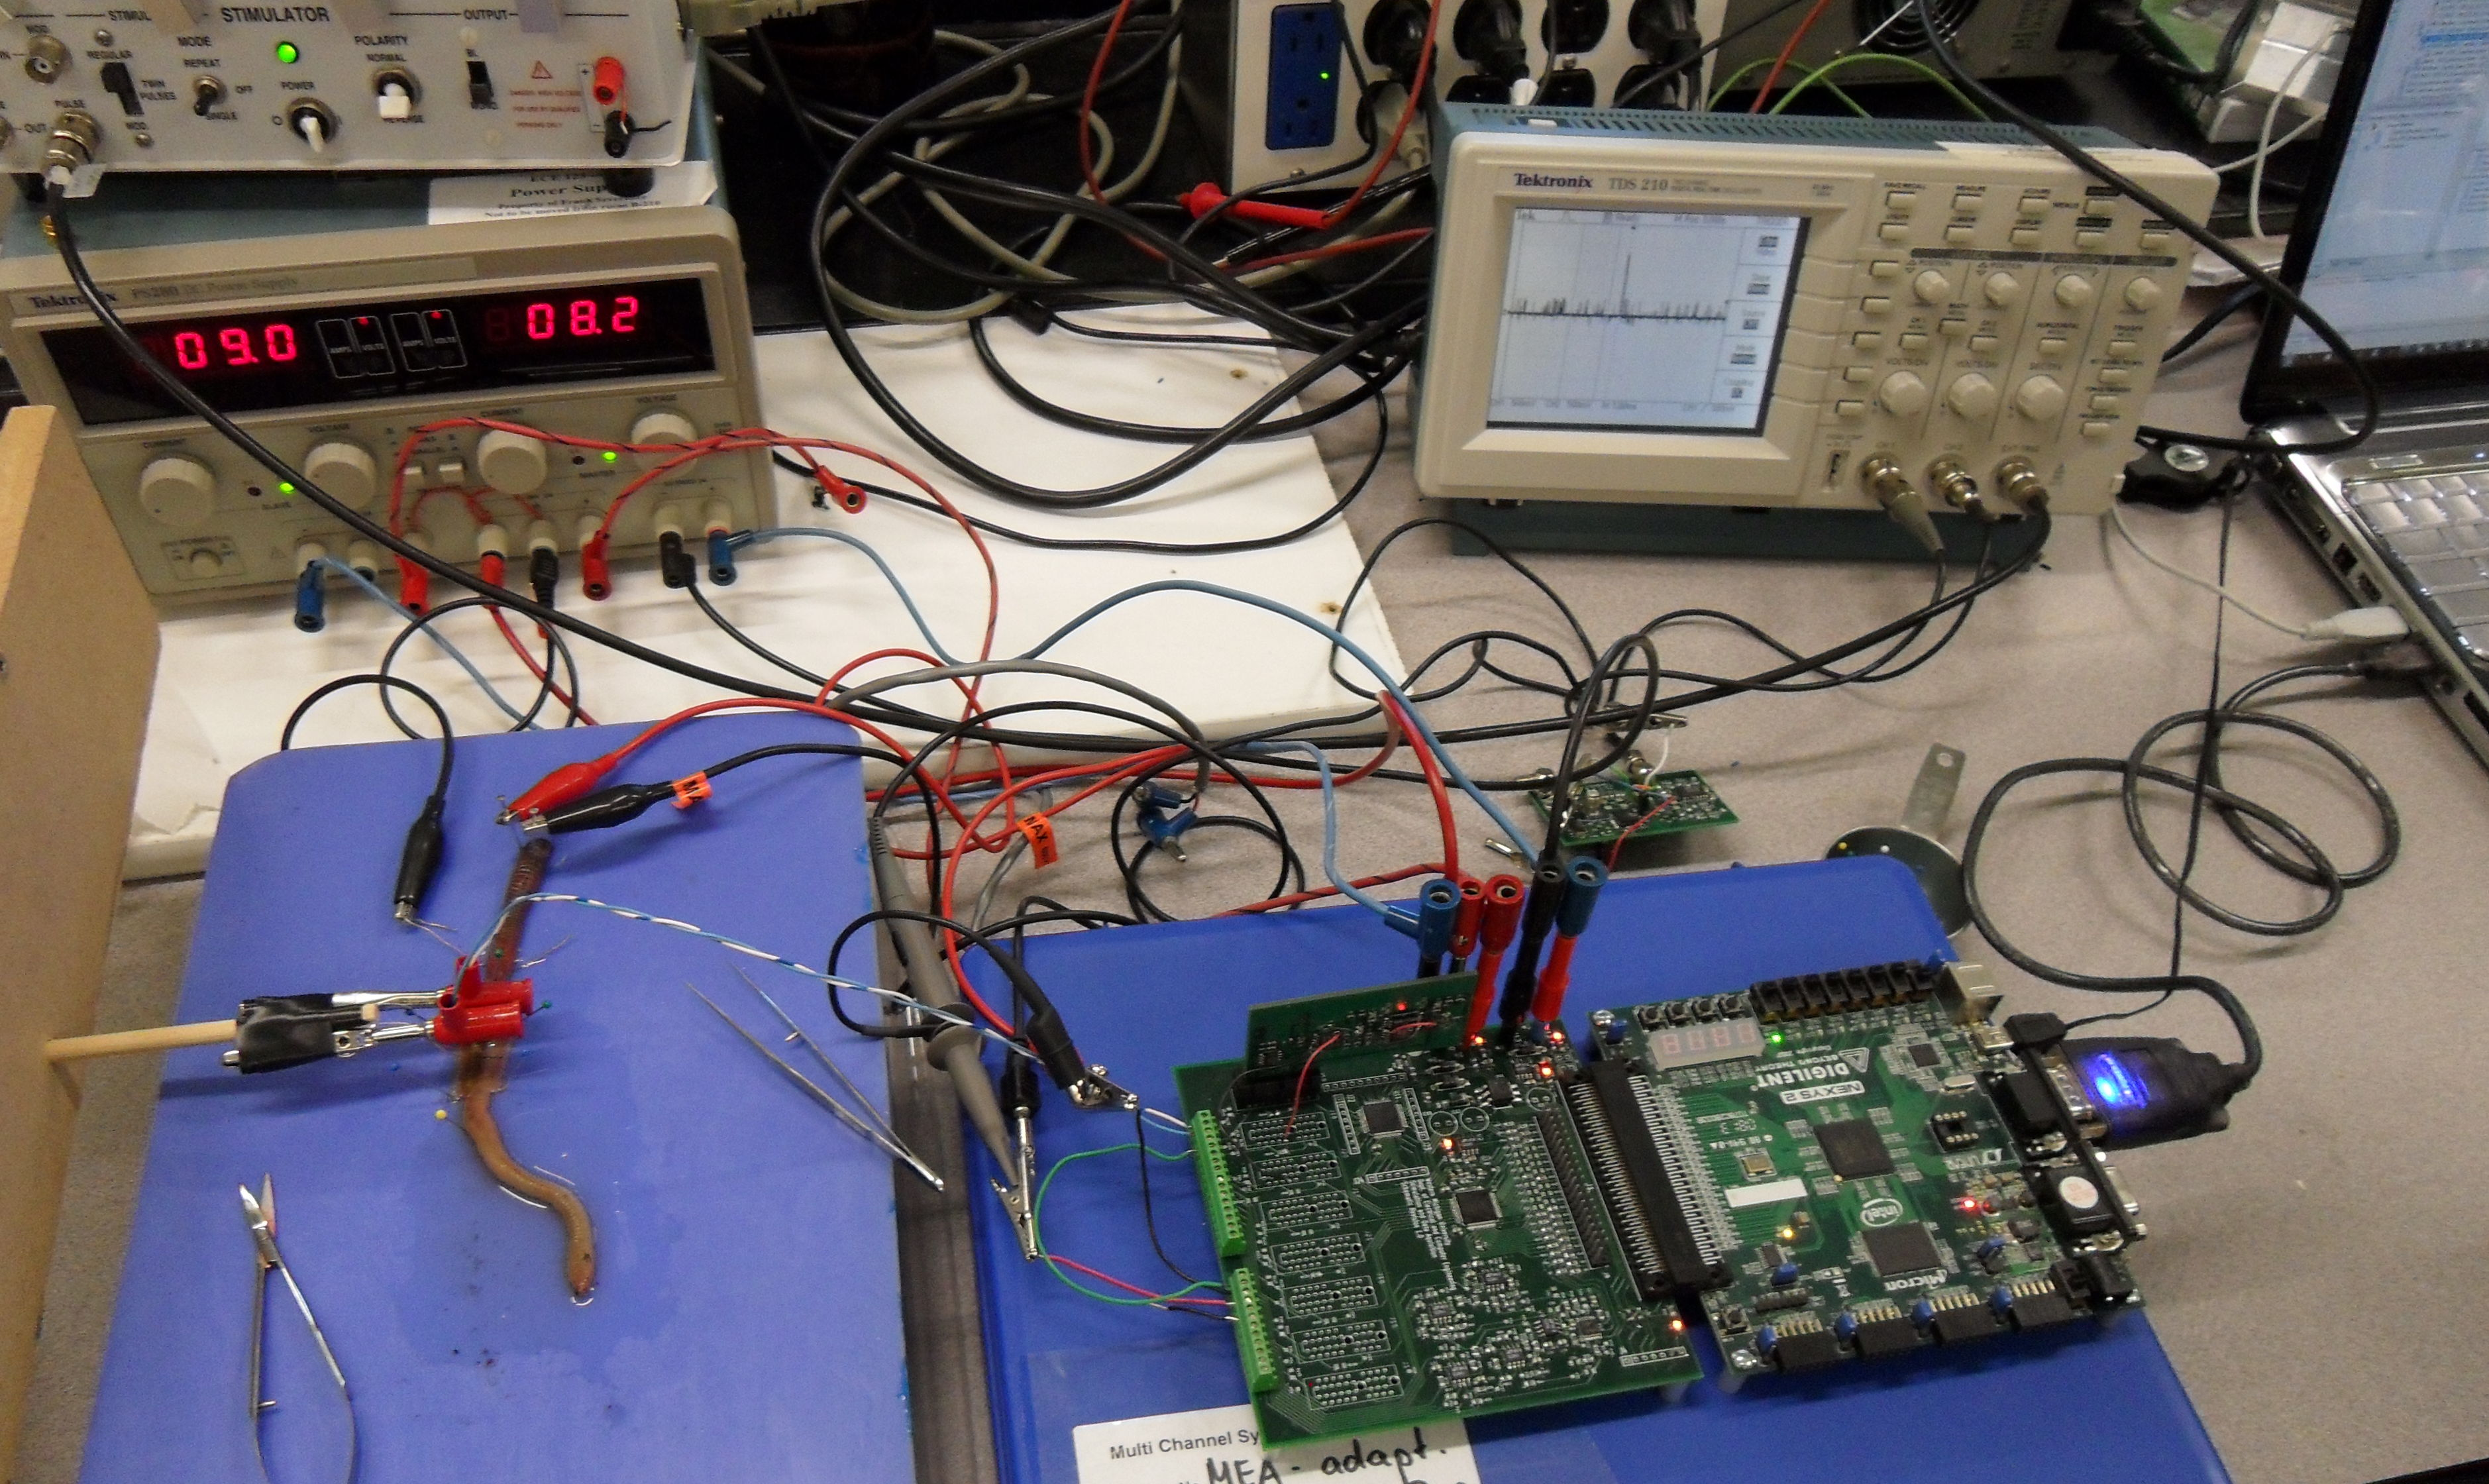
\includegraphics[width=\textwidth-0.75in]{./figures/EWSetupPic} 
	\caption{The Data Acquisition and Stimulation System connected in parallel with a previously validated recording system\label{fig:EWSetupPic}}
	\end{singlespace}
\end{figure}

Data recorded from a $2.0\unit{V}$ stimulation pulse produced a median giant response similar to those seen in~\cite{StahlMSEE} and~\cite{EllingerMSEE}.  Data from the previously validated Preamp and the oscilloscope was plotted on top of the data from the Data Acquisition and Stimulation System using a GNU Octave script.  Data from the oscilloscope and the Data Acquisition and Stimulation System can be seen in Figure~\ref{fig:EWMedResp} and the data appears to be in very close agreement.

\begin{figure}[H]
	\begin{singlespace}
	\centering 
		\resizebox{\textwidth-0.5in}{!}{% GNUPLOT: LaTeX picture with Postscript
\begingroup
  \makeatletter
  \providecommand\color[2][]{%
    \GenericError{(gnuplot) \space\space\space\@spaces}{%
      Package color not loaded in conjunction with
      terminal option `colourtext'%
    }{See the gnuplot documentation for explanation.%
    }{Either use 'blacktext' in gnuplot or load the package
      color.sty in LaTeX.}%
    \renewcommand\color[2][]{}%
  }%
  \providecommand\includegraphics[2][]{%
    \GenericError{(gnuplot) \space\space\space\@spaces}{%
      Package graphicx or graphics not loaded%
    }{See the gnuplot documentation for explanation.%
    }{The gnuplot epslatex terminal needs graphicx.sty or graphics.sty.}%
    \renewcommand\includegraphics[2][]{}%
  }%
  \providecommand\rotatebox[2]{#2}%
  \@ifundefined{ifGPcolor}{%
    \newif\ifGPcolor
    \GPcolorfalse
  }{}%
  \@ifundefined{ifGPblacktext}{%
    \newif\ifGPblacktext
    \GPblacktexttrue
  }{}%
  % define a \g@addto@macro without @ in the name:
  \let\gplgaddtomacro\g@addto@macro
  % define empty templates for all commands taking text:
  \gdef\gplbacktext{}%
  \gdef\gplfronttext{}%
  \makeatother
  \ifGPblacktext
    % no textcolor at all
    \def\colorrgb#1{}%
    \def\colorgray#1{}%
  \else
    % gray or color?
    \ifGPcolor
      \def\colorrgb#1{\color[rgb]{#1}}%
      \def\colorgray#1{\color[gray]{#1}}%
      \expandafter\def\csname LTw\endcsname{\color{white}}%
      \expandafter\def\csname LTb\endcsname{\color{black}}%
      \expandafter\def\csname LTa\endcsname{\color{black}}%
      \expandafter\def\csname LT0\endcsname{\color[rgb]{1,0,0}}%
      \expandafter\def\csname LT1\endcsname{\color[rgb]{0,1,0}}%
      \expandafter\def\csname LT2\endcsname{\color[rgb]{0,0,1}}%
      \expandafter\def\csname LT3\endcsname{\color[rgb]{1,0,1}}%
      \expandafter\def\csname LT4\endcsname{\color[rgb]{0,1,1}}%
      \expandafter\def\csname LT5\endcsname{\color[rgb]{1,1,0}}%
      \expandafter\def\csname LT6\endcsname{\color[rgb]{0,0,0}}%
      \expandafter\def\csname LT7\endcsname{\color[rgb]{1,0.3,0}}%
      \expandafter\def\csname LT8\endcsname{\color[rgb]{0.5,0.5,0.5}}%
    \else
      % gray
      \def\colorrgb#1{\color{black}}%
      \def\colorgray#1{\color[gray]{#1}}%
      \expandafter\def\csname LTw\endcsname{\color{white}}%
      \expandafter\def\csname LTb\endcsname{\color{black}}%
      \expandafter\def\csname LTa\endcsname{\color{black}}%
      \expandafter\def\csname LT0\endcsname{\color{black}}%
      \expandafter\def\csname LT1\endcsname{\color{black}}%
      \expandafter\def\csname LT2\endcsname{\color{black}}%
      \expandafter\def\csname LT3\endcsname{\color{black}}%
      \expandafter\def\csname LT4\endcsname{\color{black}}%
      \expandafter\def\csname LT5\endcsname{\color{black}}%
      \expandafter\def\csname LT6\endcsname{\color{black}}%
      \expandafter\def\csname LT7\endcsname{\color{black}}%
      \expandafter\def\csname LT8\endcsname{\color{black}}%
    \fi
  \fi
  \setlength{\unitlength}{0.0500bp}%
  \begin{picture}(11520.00,8640.00)%
    \gplgaddtomacro\gplbacktext{%
      \colorrgb{0.00,0.00,0.00}%
      \put(860,1380){\makebox(0,0)[r]{\strut{}-0.4}}%
      \colorrgb{0.00,0.00,0.00}%
      \put(860,2860){\makebox(0,0)[r]{\strut{}-0.2}}%
      \colorrgb{0.00,0.00,0.00}%
      \put(860,4339){\makebox(0,0)[r]{\strut{}0}}%
      \colorrgb{0.00,0.00,0.00}%
      \put(860,5819){\makebox(0,0)[r]{\strut{}0.2}}%
      \colorrgb{0.00,0.00,0.00}%
      \put(860,7299){\makebox(0,0)[r]{\strut{}0.4}}%
      \colorrgb{0.00,0.00,0.00}%
      \put(1905,440){\makebox(0,0){\strut{}0}}%
      \colorrgb{0.00,0.00,0.00}%
      \put(3756,440){\makebox(0,0){\strut{}2}}%
      \colorrgb{0.00,0.00,0.00}%
      \put(5607,440){\makebox(0,0){\strut{}4}}%
      \colorrgb{0.00,0.00,0.00}%
      \put(7458,440){\makebox(0,0){\strut{}6}}%
      \colorrgb{0.00,0.00,0.00}%
      \put(9308,440){\makebox(0,0){\strut{}8}}%
      \colorrgb{0.00,0.00,0.00}%
      \put(11159,440){\makebox(0,0){\strut{}10}}%
      \colorrgb{0.00,0.00,0.00}%
      \put(160,4339){\rotatebox{90}{\makebox(0,0){\strut{}Voltage ($V$)}}}%
      \colorrgb{0.00,0.00,0.00}%
      \put(6069,140){\makebox(0,0){\strut{}Time ($ms$)}}%
      \csname LTb\endcsname%
      \put(6069,8339){\makebox(0,0){\strut{}Response to $2V$ Stimulation}}%
    }%
    \gplgaddtomacro\gplfronttext{%
      \csname LTb\endcsname%
      \put(10256,7876){\makebox(0,0)[r]{\strut{}Oscilloscope Data}}%
      \csname LTb\endcsname%
      \put(10256,7676){\makebox(0,0)[r]{\strut{}ADC Data}}%
      \colorrgb{0.00,0.00,0.00}%
      \put(3987,3230){\makebox(0,0)[l]{\strut{}Stimulus Artifact}}%
      \put(4913,6189){\makebox(0,0)[l]{\strut{}Median Giant Response}}%
    }%
    \gplbacktext
    \put(0,0){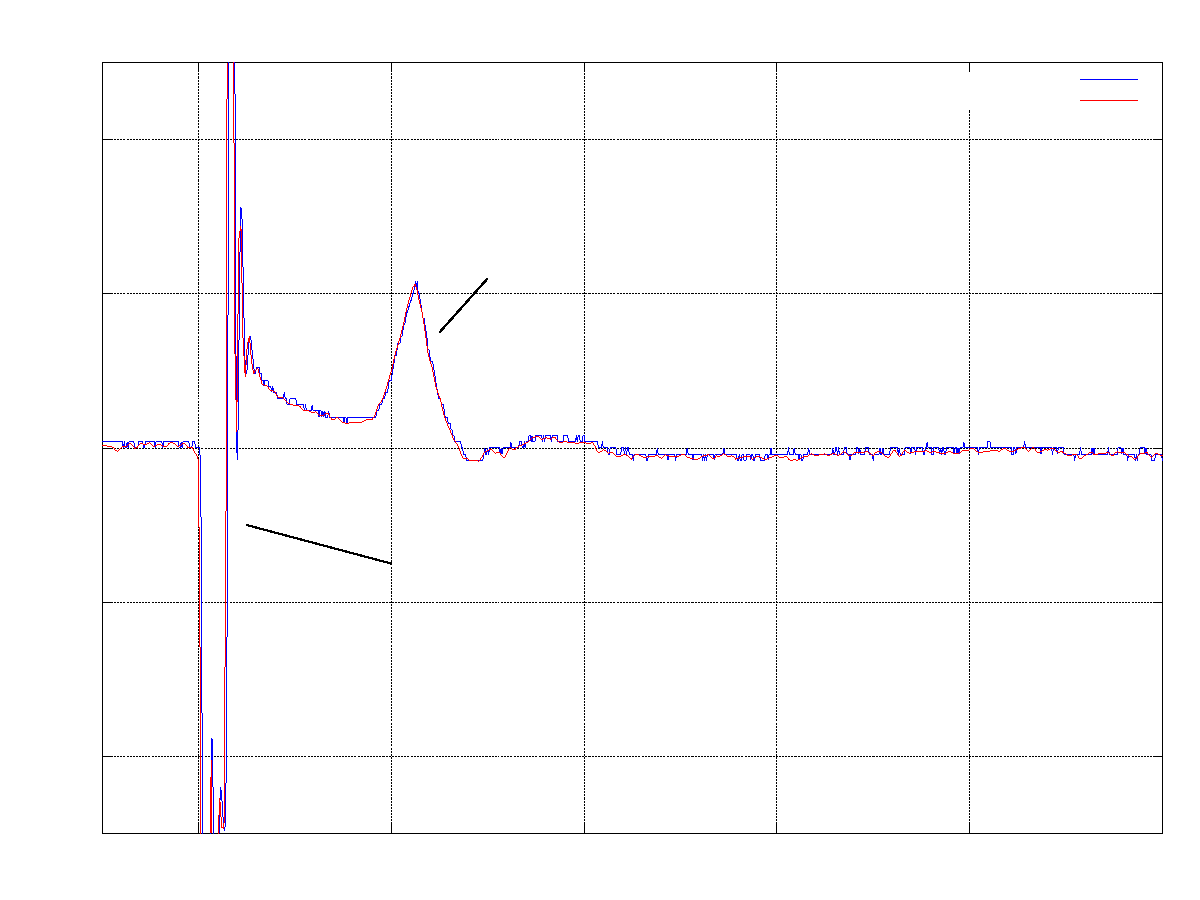
\includegraphics{median}}%
    \gplfronttext
  \end{picture}%
\endgroup
}
	\caption{Earthworm response to $2.0\unit{V}$ stimulation pulse generated by the Data Acquisition and Stimulation System with data recorded by the oscilloscope and by the ADC on the Data Acquisition and Stimulation System\label{fig:EWMedResp}}
	\end{singlespace}
\end{figure}

Data recorded from a $3.5\unit{V}$ stimulation pulse produced median and lateral giant responses similar to those seen in~\cite{StahlMSEE} and~\cite{EllingerMSEE}.  The data shown in Figure~\ref{fig:EWLatResp} exhibits close agreement between the Data Acquisition and Stimulation System and the previously validated Preamp.

\begin{figure}[H]
	\begin{singlespace}
	\centering 
		\resizebox{\textwidth-0.5in}{!}{% GNUPLOT: LaTeX picture with Postscript
\begingroup
  \makeatletter
  \providecommand\color[2][]{%
    \GenericError{(gnuplot) \space\space\space\@spaces}{%
      Package color not loaded in conjunction with
      terminal option `colourtext'%
    }{See the gnuplot documentation for explanation.%
    }{Either use 'blacktext' in gnuplot or load the package
      color.sty in LaTeX.}%
    \renewcommand\color[2][]{}%
  }%
  \providecommand\includegraphics[2][]{%
    \GenericError{(gnuplot) \space\space\space\@spaces}{%
      Package graphicx or graphics not loaded%
    }{See the gnuplot documentation for explanation.%
    }{The gnuplot epslatex terminal needs graphicx.sty or graphics.sty.}%
    \renewcommand\includegraphics[2][]{}%
  }%
  \providecommand\rotatebox[2]{#2}%
  \@ifundefined{ifGPcolor}{%
    \newif\ifGPcolor
    \GPcolorfalse
  }{}%
  \@ifundefined{ifGPblacktext}{%
    \newif\ifGPblacktext
    \GPblacktexttrue
  }{}%
  % define a \g@addto@macro without @ in the name:
  \let\gplgaddtomacro\g@addto@macro
  % define empty templates for all commands taking text:
  \gdef\gplbacktext{}%
  \gdef\gplfronttext{}%
  \makeatother
  \ifGPblacktext
    % no textcolor at all
    \def\colorrgb#1{}%
    \def\colorgray#1{}%
  \else
    % gray or color?
    \ifGPcolor
      \def\colorrgb#1{\color[rgb]{#1}}%
      \def\colorgray#1{\color[gray]{#1}}%
      \expandafter\def\csname LTw\endcsname{\color{white}}%
      \expandafter\def\csname LTb\endcsname{\color{black}}%
      \expandafter\def\csname LTa\endcsname{\color{black}}%
      \expandafter\def\csname LT0\endcsname{\color[rgb]{1,0,0}}%
      \expandafter\def\csname LT1\endcsname{\color[rgb]{0,1,0}}%
      \expandafter\def\csname LT2\endcsname{\color[rgb]{0,0,1}}%
      \expandafter\def\csname LT3\endcsname{\color[rgb]{1,0,1}}%
      \expandafter\def\csname LT4\endcsname{\color[rgb]{0,1,1}}%
      \expandafter\def\csname LT5\endcsname{\color[rgb]{1,1,0}}%
      \expandafter\def\csname LT6\endcsname{\color[rgb]{0,0,0}}%
      \expandafter\def\csname LT7\endcsname{\color[rgb]{1,0.3,0}}%
      \expandafter\def\csname LT8\endcsname{\color[rgb]{0.5,0.5,0.5}}%
    \else
      % gray
      \def\colorrgb#1{\color{black}}%
      \def\colorgray#1{\color[gray]{#1}}%
      \expandafter\def\csname LTw\endcsname{\color{white}}%
      \expandafter\def\csname LTb\endcsname{\color{black}}%
      \expandafter\def\csname LTa\endcsname{\color{black}}%
      \expandafter\def\csname LT0\endcsname{\color{black}}%
      \expandafter\def\csname LT1\endcsname{\color{black}}%
      \expandafter\def\csname LT2\endcsname{\color{black}}%
      \expandafter\def\csname LT3\endcsname{\color{black}}%
      \expandafter\def\csname LT4\endcsname{\color{black}}%
      \expandafter\def\csname LT5\endcsname{\color{black}}%
      \expandafter\def\csname LT6\endcsname{\color{black}}%
      \expandafter\def\csname LT7\endcsname{\color{black}}%
      \expandafter\def\csname LT8\endcsname{\color{black}}%
    \fi
  \fi
  \setlength{\unitlength}{0.0500bp}%
  \begin{picture}(11520.00,8640.00)%
    \gplgaddtomacro\gplbacktext{%
      \colorrgb{0.00,0.00,0.00}%
      \put(860,640){\makebox(0,0)[r]{\strut{}-1.5}}%
      \colorrgb{0.00,0.00,0.00}%
      \put(860,1873){\makebox(0,0)[r]{\strut{}-1}}%
      \colorrgb{0.00,0.00,0.00}%
      \put(860,3106){\makebox(0,0)[r]{\strut{}-0.5}}%
      \colorrgb{0.00,0.00,0.00}%
      \put(860,4340){\makebox(0,0)[r]{\strut{}0}}%
      \colorrgb{0.00,0.00,0.00}%
      \put(860,5573){\makebox(0,0)[r]{\strut{}0.5}}%
      \colorrgb{0.00,0.00,0.00}%
      \put(860,6806){\makebox(0,0)[r]{\strut{}1}}%
      \colorrgb{0.00,0.00,0.00}%
      \put(860,8039){\makebox(0,0)[r]{\strut{}1.5}}%
      \colorrgb{0.00,0.00,0.00}%
      \put(1905,440){\makebox(0,0){\strut{}0}}%
      \colorrgb{0.00,0.00,0.00}%
      \put(3756,440){\makebox(0,0){\strut{}2}}%
      \colorrgb{0.00,0.00,0.00}%
      \put(5607,440){\makebox(0,0){\strut{}4}}%
      \colorrgb{0.00,0.00,0.00}%
      \put(7458,440){\makebox(0,0){\strut{}6}}%
      \colorrgb{0.00,0.00,0.00}%
      \put(9308,440){\makebox(0,0){\strut{}8}}%
      \colorrgb{0.00,0.00,0.00}%
      \put(11159,440){\makebox(0,0){\strut{}10}}%
      \colorrgb{0.00,0.00,0.00}%
      \put(160,4339){\rotatebox{90}{\makebox(0,0){\strut{}Voltage ($V$)}}}%
      \colorrgb{0.00,0.00,0.00}%
      \put(6069,140){\makebox(0,0){\strut{}Time ($ms$)}}%
      \csname LTb\endcsname%
      \put(6069,8339){\makebox(0,0){\strut{}Response to $3.5V$ Stimulation}}%
    }%
    \gplgaddtomacro\gplfronttext{%
      \csname LTb\endcsname%
      \put(10256,7876){\makebox(0,0)[r]{\strut{}Oscilloscope Data}}%
      \csname LTb\endcsname%
      \put(10256,7676){\makebox(0,0)[r]{\strut{}ADC Data}}%
      \colorrgb{0.00,0.00,0.00}%
      \put(3987,2736){\makebox(0,0)[l]{\strut{}Stimulus Artifact}}%
      \put(4913,5943){\makebox(0,0)[l]{\strut{}Median Giant Response}}%
      \put(8614,5943){\makebox(0,0)[l]{\strut{}Lateral Giant Response}}%
    }%
    \gplbacktext
    \put(0,0){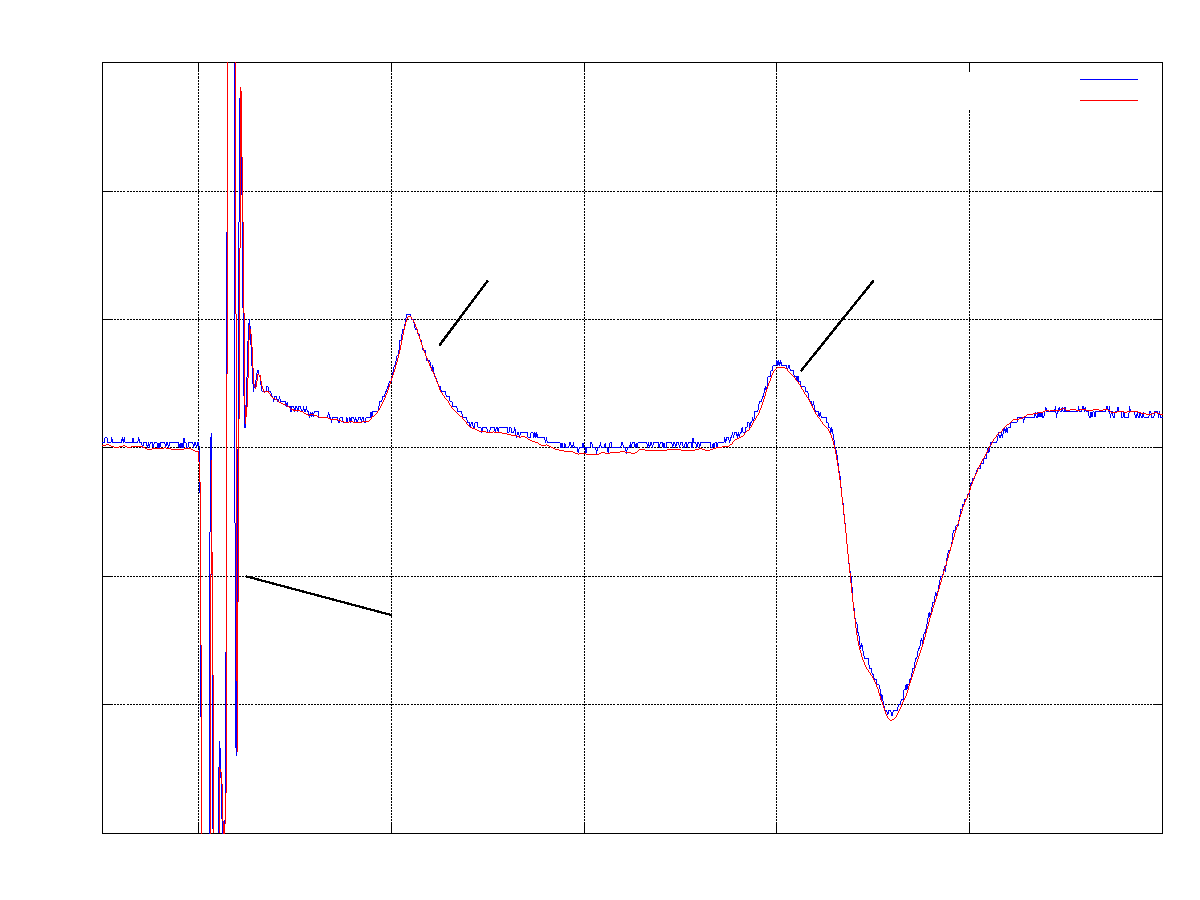
\includegraphics{lateral}}%
    \gplfronttext
  \end{picture}%
\endgroup
}
	\caption{Earthworm response to $3.5\unit{V}$ stimulation pulse generated by the Data Acquisition and Stimulation System with data recorded by the oscilloscope and by the ADC on the Data Acquisition and Stimulation System\label{fig:EWLatResp}}
	\end{singlespace}
\end{figure}
